\section{Classifiers, Reduction of the dimensionality algorithms and Cross Validation}
Classifying is called to the task of sign a a category to a object. The classification task is based in the features of the object obtained of the feature extractor \cite{Duda}, that in the particular case of this thesis is the output of a convolutional neural network.\\

The output of the convolutional neural network could be bigger enough and some features could not be relevant for the classification. To solve the speed and robustness issues that could appear because of the quantity of features \cite{PCAvsLDA}, techniques to reduce the dimensionality are used.\\

Classifiers must be customized to each problem, to find the optimal parameters for each occasion, cross validation technique has been used.\\

\subsection{Classifiers}
In this section, the classifiers used along the thesis are described.\\

\subsubsection{Logistic Regression}
Logistic regression is a probabilistic and a linear classifier. It is customized by a weight matrix \textit{W} and a bias vector \textit{b}.\\

The logistic regression weights and bias define a linear hyperplane which is the decision boundary of the classes. In order to find the parameters, the Maximum likelihood estimation is used during training \cite{ClassifiersReview}:\\

\begin{equation}
\prod_{i=1}^{n}P(y_i|X_i,W,b)
\end{equation}

Given a input vector \textit{x}, which belongs to the \textit{i} class (a value of a stochastic variable \textit{Y}), its probability could be described as follows:

\begin{equation}
P(Y=i|x,W,b) = \frac{e^{W_ix+b_i}}{\sum_j e^{W_ix+b_i}}
\end{equation}

The class of a new sample (\textit{y\_{pred}}) would be classify as:

\begin{equation}
y_{pred} = argmax_{i}P(y_i|X_i,W,b)
\end{equation}

That is that the sample would belong to a class depending on position in the space with respect to the hyperplane that separates the classes.\\

\subsubsection{Support Vector Machine}
Support Vector Machine (SVM) is a two-class classifier. The smallest generalization error is linked to the \textit{margin} concept. Margin is the perpendicular distance between the closest sample of the database and the calculate hyperplane \cite{MachineLearning}. An hyperplane is optimal if the margin is the maximum and this margin is calculated (as the same way as logistic regression):\\

\begin{equation}
\underset{w b}{\operatorname{arg\,max}}\left \{ \frac{1}{||W||} \underset{n}{\operatorname{min}}[t_{n}(W^T \phi (X_n)+b)]   \right \}
\end{equation}


Where \textit{w, b} are the parameters that should be optimized in order to maximize the distance. \textit{$t_n$} are the training samples. $\phi$ is a fixed feature-space transformation, \textit{b} is the bias parameter.\\

\begin{figure}[htb]
\centering
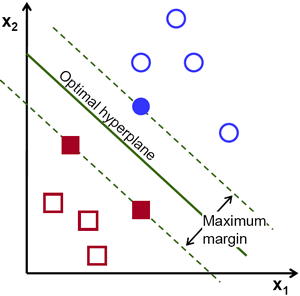
\includegraphics[width=0.5\textwidth]{images_miscelaneus/svm.png}
\caption{Optimal hyperplane and the decision boundary. Image obtained from \cite{SVMimage}} \label{fig:SVM}
\end{figure}

In figure \ref{fig:SVM} the optimal hyperplane between two classes are represented with its corresponding margin. In this example the two classes are well differentiated. This image has been obtained from \cite{SVMimage}.\\

Based on estimate the hyperplane that the distance between classes, the closest vectors of each class, is maximized \cite{SVM1, MachineLearning}. In practice, the margin is determined by \textit{C}, a parameter that should be chosen by user to get the optimal margin.\\

The SVM performance is join to a kernel function which allows variability in nonlinearity and flexibility in the model \cite{ClassifiersReview, practicalguideSVM}. There are many kernels (polynomial, sigmoid...), but the two used are described:

\begin{enumerate}
\item linear: $ K(x_{i},x_{j}) = x_i^T)x_j$.
\item radial basis function (RBF): $K(x_{i},x_{j}) = exp(-\gamma||x_i-x_j||^2), \gamma>0$ 
\end{enumerate}
 

\subsubsection{K Nearest Neighbours}
K- Nearest Neighbour (KNN) is a generative and non parametric classifier. For classifying, the density estimation procedure is used. The difference between this classifiers and others used is this algorithm uses the data directly for classification, without building a model first \cite{ClassifiersReview}. The density function is determined by the form \cite{MachineLearning}:
\begin{equation}
p(x) = \frac{K}{N V}
\end{equation}

Where \textit{K} is the number of points inside the region \textit{R} whose volume is \textit{V} and \textit{N} is the number of total samples or observations.\\

This classifiers uses the observation directly to classify and needs all the samples to predict a new one. The probability of a sample \textit{x} belonging to a class \textit{$C_k$} is defined by \cite{MachineLearning}:
\begin{equation}
p(x|C_k) = \frac{K_k}{N_k V}
\end{equation}

Where $N_k$ are the observations of a class $C_k$ and $K_k$ of it class points are contained in the volume \textit{V}.\\

The \textit{K} value is fixed, should be calculated and optimized by user of each application.\\

\subsubsection{Decision Tree}
Decision Tree classifier is based in a natural classification based in a sequence of true/false or yes/no questions \cite{Duda}.\\




\subsection{Dimensionality reduction algorithms}
The objective of those algorithms is transform the characteristic vector into another characteristic vector but whit a lower dimensionality. Linear methods, that projects the dimensional data onto an another space whose dimensionality is lower \cite{Duda}, have been used. The two techniques, the most common used, are described and used along the thesis.\\
\subsubsection{Linear Discriminant Analysis}
Linear Discriminant Analysis (LDA) looks for the vectors in the space that best discriminate among classes \cite{PCAvsLDA}.

\subsubsection{Principal Component Analysis}
Principal Component Analysis (PCA) uses a subspace in which the the variance direction among basis vectors is maximum in the original space \cite{PCAvsLDA}

\subsection{Cross Validation}
